\documentclass[11pt]{article}
\usepackage{amsmath, amssymb, amsthm}
\usepackage[retainorgcmds]{IEEEtrantools}

\usepackage[pdftex]{graphicx}
\usepackage{tikz}
\usepackage{circuitikz}
\usetikzlibrary{intersections}

\usepackage{fancyhdr}

%Listings stuff
\usepackage{listings}
\usepackage{lstautogobble}
\usepackage{color}

\definecolor{gray}{rgb}{0.5,0.5,0.5}
\lstset{
basicstyle={\small\ttfamily},
tabsize=3,
numbers=left,
numbersep=5pt,
numberstyle=\tiny\color{gray},
stepnumber=2,
breaklines=true,
boxpos=t
}

%Format stuff
\pagestyle{fancy}
\headheight 35pt

%Header info
\chead{\Large \textbf{Huffman Codes}}
\lhead{}
\rhead{}

\begin{document}
\section{Encoding}
	Huffman coding is a lossless ecoding algorithm that encodes an alphabet into a \textbf{prefix code}, a mapping of codewords to characters so that no codeword is a prefix of another. The encoded alphabet can be represented as a binary tree with all letters on the leaves.
	
	\begin{center}
	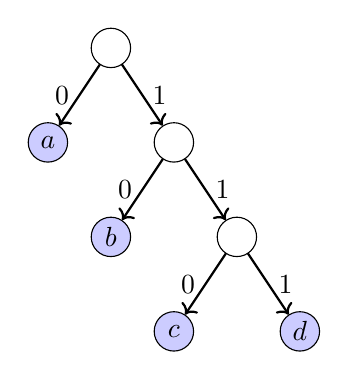
\begin{tikzpicture}
		[scale=.8,line cap=round,
		%Styles
		axes/.style=,
		important line/.style={very thick},
		information text/.style={rounded corners,fill=red!10,inner sep=1ex},
		dot/.style={circle,inner sep=1pt,fill,label={#1},name=#1},
		main node/.style={circle,fill=blue!20,draw,minimum size=5mm,inner sep=0pt},					inner node/.style={circle,draw,minimum size=5mm,inner sep=0pt}
		]
		
		%Colors
		\colorlet{anglecolor}{green!50!black}	%angle arcs/lines
		
		%The graphic
		\node[inner node] (A) at (0, 0) {};
		\node[main node] (B) at (-1, -1.5) {$a$};
		\node[inner node] (C) at (1, -1.5) {};
		\node[main node] (D) at (0, -3) {$b$};
		\node[inner node] (E) at (2, -3) {};
		\node[main node] (F) at (1, -4.5) {$c$};
		\node[main node] (G) at (3, -4.5) {$d$};
		
		\path[thick,->]
			(A)	edge	node[left] {$0$}	(B)
				edge	node[right] {$1$}	(C)
			(C)	edge	node[left] {$0$}	(D)
				edge	node[right] {$1$}	(E)
			(E)	edge	node[left] {$0$}	(F)
				edge	node[right] {$1$}	(G);
	\end{tikzpicture}
	\end{center}
	
	\subparagraph{Optimal Code} If $P(x)$ is the probability of letter $x$ and $d_T(x)$ is the depth in the tree of the codeword, for an alphabet $C$, the expected encoding length for $n$ characters, which we want to minimize, is
	
	\begin{equation}
		B(T) = n\sum_{x\in C} p(x)d_T(x)
	\end{equation}
	
\section{Algorithm}
	Build the tree bottom-up, merging 2 characters into a meta-character on each step, then recurse on the 1-letter smaller alphabet with the meta-character. When merging, always pick the 2 characters with the lowest probability.
	
	\begin{lstlisting}[autogobble=true]
		for x in C:
			add x to heap Q by p(x)
			
		for i in [1, |C| - 1]:
			z = new internal tree node
			left[z] = x = extract-min(Q)
			right[z] = y = extract-min(Q)
			p(z) = p(x) + p(y)
			insert z into Q
			
		return last element in Q as root
	\end{lstlisting}
	
\section{Proof}
	\subparagraph{Claim} For $x, y \in C$ with the lowest probabilities, there exists an optimal tree with these two letters at maximum depth.
	\subparagraph{Proof} By contradiction, take $b, c, x, y \in C \mid p(b) \leq p(c), p(x) \leq p(y)$ with no loss of generality. By the claim that $x$ and $y$ have the lowest probabilities, $p(x) \leq p(b), p(y) \leq p(c)$. Now put $b, c$ at the bottom of the tree so that $d_T(b) \geq d_T(x), d_T(c) \geq d_T(y)$.
	
	\begin{center}
	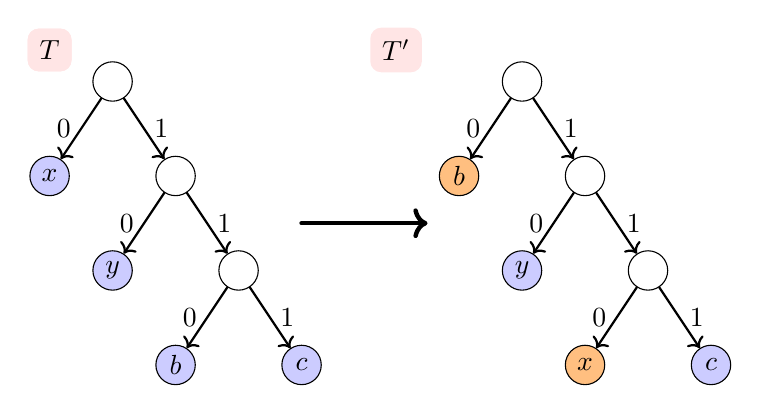
\begin{tikzpicture}
		[scale=.8,line cap=round,
		%Styles
		axes/.style=,
		important line/.style={very thick},
		information text/.style={rounded corners,fill=red!10,inner sep=1ex},
		dot/.style={circle,inner sep=1pt,fill,label={#1},name=#1},
		main node/.style={circle,fill=blue!20,draw,minimum size=5mm,inner sep=0pt},					inner node/.style={circle,draw,minimum size=5mm,inner sep=0pt}
		]
		
		%Colors
		\colorlet{anglecolor}{green!50!black}	%angle arcs/lines
		
		%The graphic
		\node[inner node] (A) at (0, 0) {};
		\node[main node] (B) at (-1, -1.5) {$x$};
		\node[inner node] (C) at (1, -1.5) {};
		\node[main node] (D) at (0, -3) {$y$};
		\node[inner node] (E) at (2, -3) {};
		\node[main node] (F) at (1, -4.5) {$b$};
		\node[main node] (G) at (3, -4.5) {$c$};
		
		\node[information text] at (-1, .5) {$T$};		
		
		\path[thick,->]
			(A)	edge	node[left] {$0$}	(B)
				edge	node[right] {$1$}	(C)
			(C)	edge	node[left] {$0$}	(D)
				edge	node[right] {$1$}	(E)
			(E)	edge	node[left] {$0$}	(F)
				edge	node[right] {$1$}	(G);
				
		\draw[ultra thick, ->] (3, -2.25) -- (5, -2.25);
		
		\node[information text] at (4.5, .5) {$T'$};
		
		\node[inner node] (H) at (6.5, 0) {};
		\node[main node,fill=orange!50] (I) at (5.5, -1.5) {$b$};
		\node[inner node] (J) at (7.5, -1.5) {};
		\node[main node] (K) at (6.5, -3) {$y$};
		\node[inner node] (L) at (8.5, -3) {};
		\node[main node,fill=orange!50] (M) at (7.5, -4.5) {$x$};
		\node[main node] (N) at (9.5, -4.5) {$c$};
		
		\node[information text] at (-1, .5) {$T$};		
		
		\path[thick,->]
			(H)	edge	node[left] {$0$}	(I)
				edge	node[right] {$1$}	(J)
			(J)	edge	node[left] {$0$}	(K)
				edge	node[right] {$1$}	(L)
			(L)	edge	node[left] {$0$}	(M)
				edge	node[right] {$1$}	(N);
	\end{tikzpicture}
	\end{center}
	
	Swap the positions of $x$ and $b$ in the tree to obtain the new tree $T'$. The cost change from $T$ to $T'$ is given by:
	
	\begin{IEEEeqnarray}{rCl}
		B(T') & = & B(T) - p(x)d_T(x) + p(x)d_T(b) - p(b)d_T(b) + p(b)d_T(x)\\
		& = & B(T) + p(x)(d_T(b) - d_T(x)) - p(b)(d_T(b)-d_T(x))\\
		& = & B(T) - (p(b) - p(x))(d_T(b) - d_T(x))
	\end{IEEEeqnarray}
	In the analysis above, we fixed that $p(x) \leq p(b)$ and $d_T(x) \leq d_T(b)$, so therefore $B(T') \leq B(T)$. By a similar exchange argument for $y$, this proves that there exists some optimal tree with $x$ and $y$ at the deepest level.
	
	\subparagraph{Claim} Huffman's algorithm always produces an optimal tree.
	
	\subparagraph{Proof} Use induction. The base case $n=1$ is trivially correct, and by the inductive hypothesis we assume correctness on $n-1$ characters.
	
	Given a tree for $n$ characters such that $x, y$ are the lowest probability letters, we know that they are at the bottom of the optimal solution. Now replace $x, y$ with $z$ so that $p(z) = p(x) + p(y)$, as in the algorithm so that now $|C'| = n - 1$.
	
	Consider that \textit{any} prefix tree $T$ for $C'$ has $z$ as a leaf node (by definition). Replace this leaf node with an internal node branching out to two new leaves $x$ and $y$. The cost change is:
	
	\begin{IEEEeqnarray}{rCl}
		B(T') & = & B(T) - p(z)d_T(z) + p(x)(d_T(z) + 1) + p(y)(d_T(z) + 1)\\
		& = & B(T) + (p(x) + p(y))
	\end{IEEEeqnarray}
	
	By the inductive hypothesis, $B(T)$ is minimal. Because we picked $x, y$ so that their sum would be the smallest possible out of the alphabet, $B(T')$ is optimal as well, which means Huffman's algorithm always produces a minimal prefix code.
%	\begin{center}
%	\begin{tikzpicture}
%		[scale=3,line cap=round,
%		%Styles
%		axes/.style=,
%		important line/.style={very thick},
%		information text/.style={rounded corners,fill=red!10,inner sep=1ex},
%		dot/.style={circle,inner sep=1pt,fill,label={#1},name=#1}			
%		]
%		
%		%Colors
%		\colorlet{anglecolor}{green!50!black}	%angle arcs/lines
%		
%		%The graphic
%	\end{tikzpicture}
%	\end{center}

%	\begin{figure}[htb]
%		\centering
%		\includegraphics[width=0.8\textwidth]{filename.eps}
%		\caption{Caption.}
%		\label{fig:figure}
%	\end{figure}

%		\def\enotesize{\normalsize}
%		\theendnotes
\end{document}